\chapter{Prototype Implementation}
\label{cha:implementation}
\vspace{0.4 cm}

This chapter presents which components of the system have been implemented and how.
Only a subset of the components of the designed architecture in chapter~\ref{cha:system} have been implemented.
This is because a prototype was developed as a Proof of Concept (PoC) with a focus on key components for verifying the system functionality which was then possible to verify the performance of the models.
The rest was not implemented since it was not crucial for having a working system, in fact, the overall architecture was designed in order to build a working Software as a Service (SaaS) on top of the core system functionalities implemented.

The first section describes the implementation of the system's common components across the various specific use cases and the others explain the implementation details of the use case-specific modules.
After this chapter, it will be clear how the system prototype was implemented for testing and validation, which are discussed in the next chapter.


\section{System's common components}
\label{sec:componentsimpl}
\vspace{0.2 cm}

The effectively implemented components of the architecture designed for the proposed system is described in figure~\ref{fig:implementationcomponents}.
Describe the implementation of the system's common components ...
\begin{itemize}
  \item ML model interface: interface with the ML models storage for storing the ML models and retrieving the stored ones making them available (interface to MLflow model storage using a Python client was thought of as a possible interface for the complete system integration);
  \item Model training task: trains new models based on available data;
  \item Forecasting task: forecasts future data using all the available models.
\end{itemize}

\begin{figure}[H]
\centering
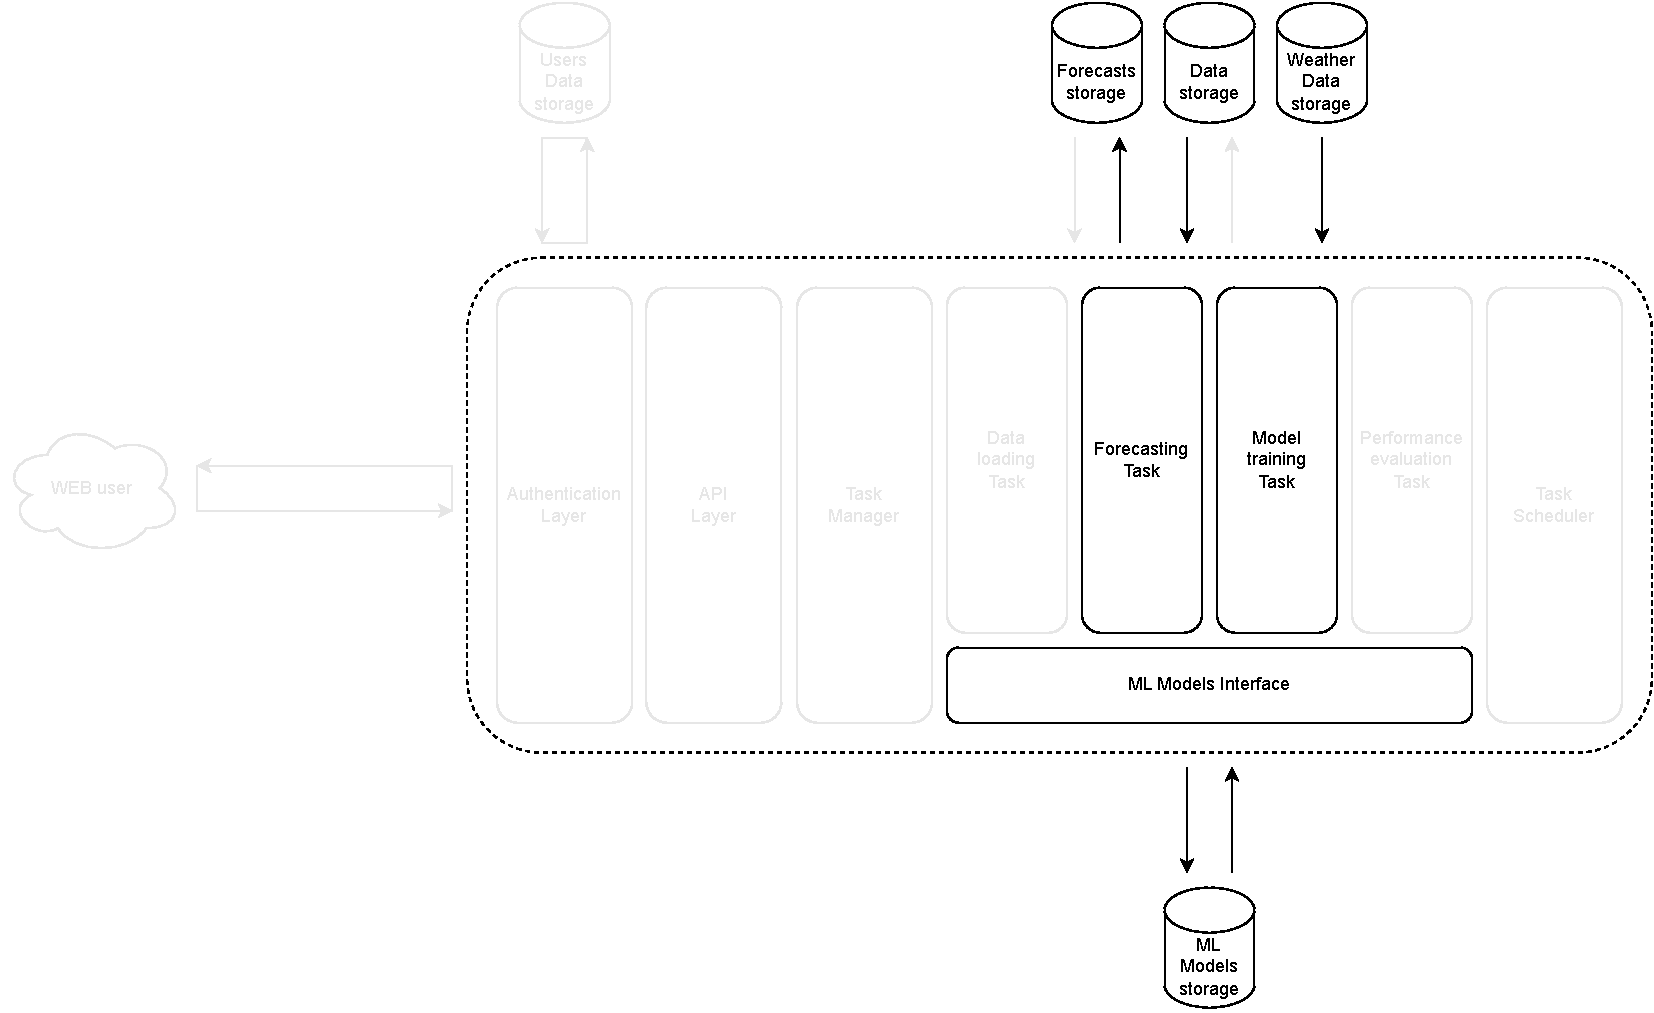
\includegraphics[width=0.9\textwidth]{images/implementation_components}
\caption{The effectively implemented components of the architecture designed for the proposed system.}
\label{fig:implementationcomponents}
\end{figure}

The system interacts with the following external components:
\begin{itemize}
  \item Data storage: data are stored as CSV files (InfluxDB was thought of as a possible database for the complete system integration);
  \item Weather data storage: weather data are stored as a JSON file and is manually obtained from Weatherbit\footnote{ \url{https://www.weatherbit.io/} } APIs (InfluxDB was thought of as a possible database for the complete system integration with an automatic download using Weatherbit APIs);
  \item ML models storage: ML models are stored as pickle files (MLflow was thought of as a possible model storage for the complete system integration);
  \item Forecasts storage: forecasts are stored as CSV files (InfluxDB was thought of as a possible database for the complete system integration).
\end{itemize}

The interactions among the effectively implemented components of the architecture designed for the proposed system are described in figure~\ref{fig:implementationinteractions}.

\begin{figure}[H]
\centering
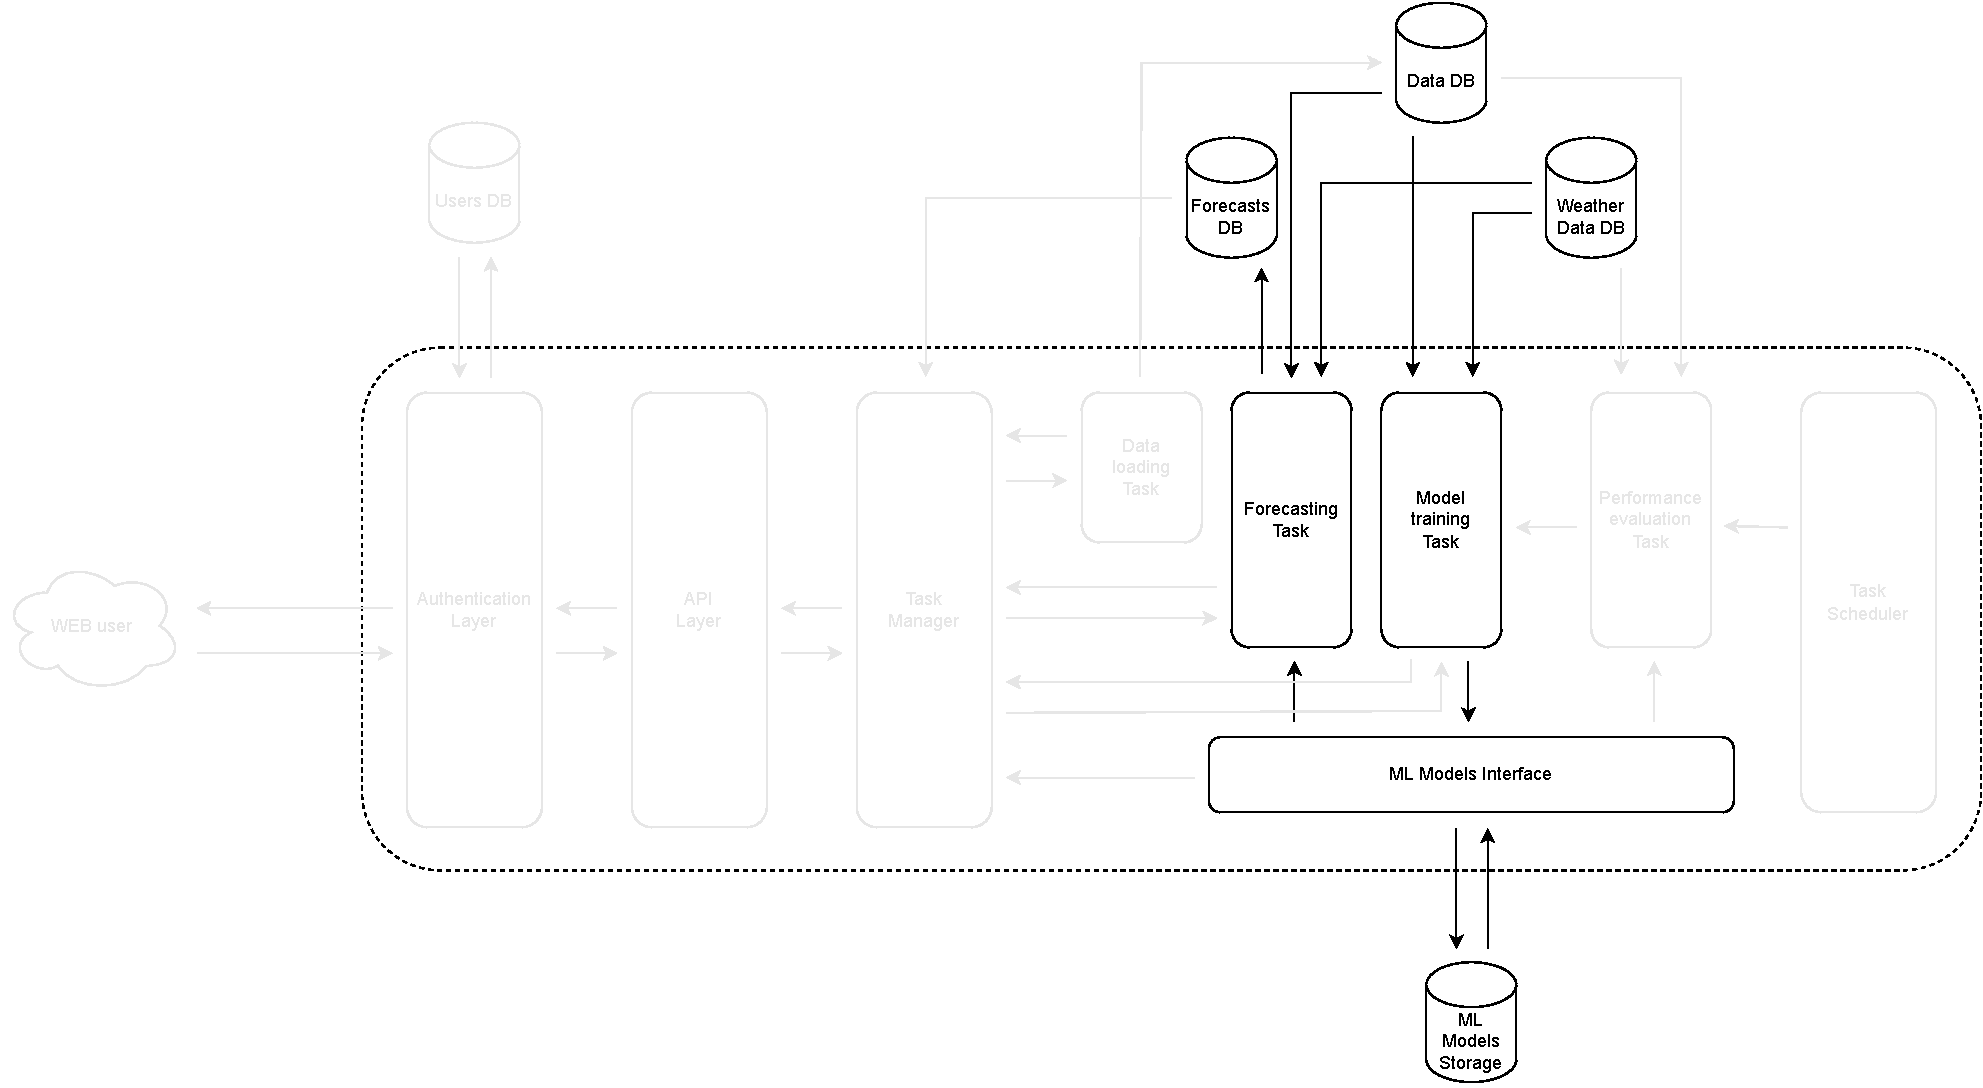
\includegraphics[width=1\textwidth]{images/implementation_interactions}
\caption{The interactions among the effectively implemented components of the architecture designed for the proposed system.}
\label{fig:implementationinteractions}
\end{figure}


\section{Electricity demand forecasting models}
\label{sec:demandimpl}
\vspace{0.2 cm}

Describe the implementation of the electricity demand forecasting models ...
\begin{itemize}
  \item data preprocessing: describe the specific preprocessing;
  \item models training: describe the training for all the specific models;
  \item prediction: describe the prediction for all the specific models.
\end{itemize}

Built models:
\begin{itemize}
  \item baseline approaches which consider repeating past days and weeks;
  \item ARIMA;
  \item hist gradient boosting regressor;
  \item extreme gradient boosting regressor;
  \item prophet;
  \item LSTM;
  \item GRU;
  \item CNN;
  \item combination of different techniques;
  \item TFT;
  \item AutoML approach.
\end{itemize}

The ARIMA model was developed using the pmdarima\footnote{ \url{http://alkaline-ml.com/pmdarima/} } library.
The hist gradient boosting regressor model was developed using the scikit-learn\footnote{ \url{https://scikit-learn.org/} } library;
The extreme gradient boosting regressor model was developed using the XGBoost\footnote{ \url{https://xgboost.readthedocs.io/} } library;
The prophet model was developed using the prophet\footnote{ \url{https://facebook.github.io/prophet/} } library;
The LSTM, GRU, and CNN models were developed using the keras\footnote{ \url{https://keras.io/} } library;
The TFT model was developed using the pytorch-forecasting\footnote{ \url{https://pytorch-forecasting.readthedocs.io/} } library;
The AutoML approach was based on Auto-PyTorch\footnote{ \url{https://automl.github.io/Auto-PyTorch/master/} }.


\section{Consumption baseline forecasting models}
\label{sec:baselineimpl}
\vspace{0.2 cm}

Describe the implementation of the consumption baseline forecasting models ...
\begin{itemize}
  \item data preprocessing: describe the specific preprocessing;
  \item models training: describe the training for all the specific models;
  \item prediction: describe the prediction for all the specific models.
\end{itemize}

Built models:
\begin{itemize}
  \item baseline approaches which consider repeating past days and weeks;
  \item ARIMA;
  \item hist gradient boosting regressor;
  \item extreme gradient boosting regressor;
  \item prophet;
  \item LSTM;
  \item GRU;
  \item CNN;
  \item combination of different techniques;
  \item TFT;
  \item AutoML approach.
\end{itemize}

The ARIMA model was developed using the pmdarima\footnote{ \url{http://alkaline-ml.com/pmdarima/} } library.
The hist gradient boosting regressor model was developed using the scikit-learn\footnote{ \url{https://scikit-learn.org/} } library;
The extreme gradient boosting regressor model was developed using the XGBoost\footnote{ \url{https://xgboost.readthedocs.io/} } library;
The prophet model was developed using the prophet\footnote{ \url{https://facebook.github.io/prophet/} } library;
The LSTM, GRU, and CNN models were developed using the keras\footnote{ \url{https://keras.io/} } library;
The TFT model was developed using the pytorch-forecasting\footnote{ \url{https://pytorch-forecasting.readthedocs.io/} } library;
The AutoML approach was based on Auto-PyTorch\footnote{ \url{https://automl.github.io/Auto-PyTorch/master/} }.


\section{Electricity production forecasting models}
\label{sec:productionimpl}
\vspace{0.2 cm}

Describe the implementation of the electricity production forecasting models ...
\begin{itemize}
  \item data preprocessing: describe the specific preprocessing;
  \item models training: describe the training for all the specific models;
  \item prediction: describe the prediction for all the specific models.
\end{itemize}

Built models:
\begin{itemize}
  \item baseline approaches which consider repeating past days and weeks;
  \item ARIMA;
  \item support vector regressor;
  \item hist gradient boosting regressor;
  \item extreme gradient boosting regressor;
  \item prophet;
  \item LSTM;
  \item GRU;
  \item CNN;
  \item combination of different techniques;
  \item TFT;
  \item AutoML approach.
\end{itemize}

The ARIMA model was developed using the pmdarima\footnote{ \url{http://alkaline-ml.com/pmdarima/} } library.
The support vector regressor and hist gradient boosting regressor models were developed using the scikit-learn\footnote{ \url{https://scikit-learn.org/} } library;
The extreme gradient boosting regressor model was developed using the XGBoost\footnote{ \url{https://xgboost.readthedocs.io/} } library;
The prophet model was developed using the prophet\footnote{ \url{https://facebook.github.io/prophet/} } library;
The LSTM, GRU, and CNN models were developed using the keras\footnote{ \url{https://keras.io/} } library;
The TFT model was developed using the pytorch-forecasting\footnote{ \url{https://pytorch-forecasting.readthedocs.io/} } library;
The AutoML approach was based on Auto-PyTorch\footnote{ \url{https://automl.github.io/Auto-PyTorch/master/} }.
